
\section{Existing ontology work}
\label{existingontologies}

One of the key aspects of FAIR ontologies is the active reusability of existing
ontologies.

\subsection{The Basic Formal Ontology}

Some description about BFO and why we use the 2020 version.

\subsection{The Open Energy Ontology}

OEO section

\begin{figure}[h]
    \caption{Open energy ontology electric vehicle commitments.}
    \centering
    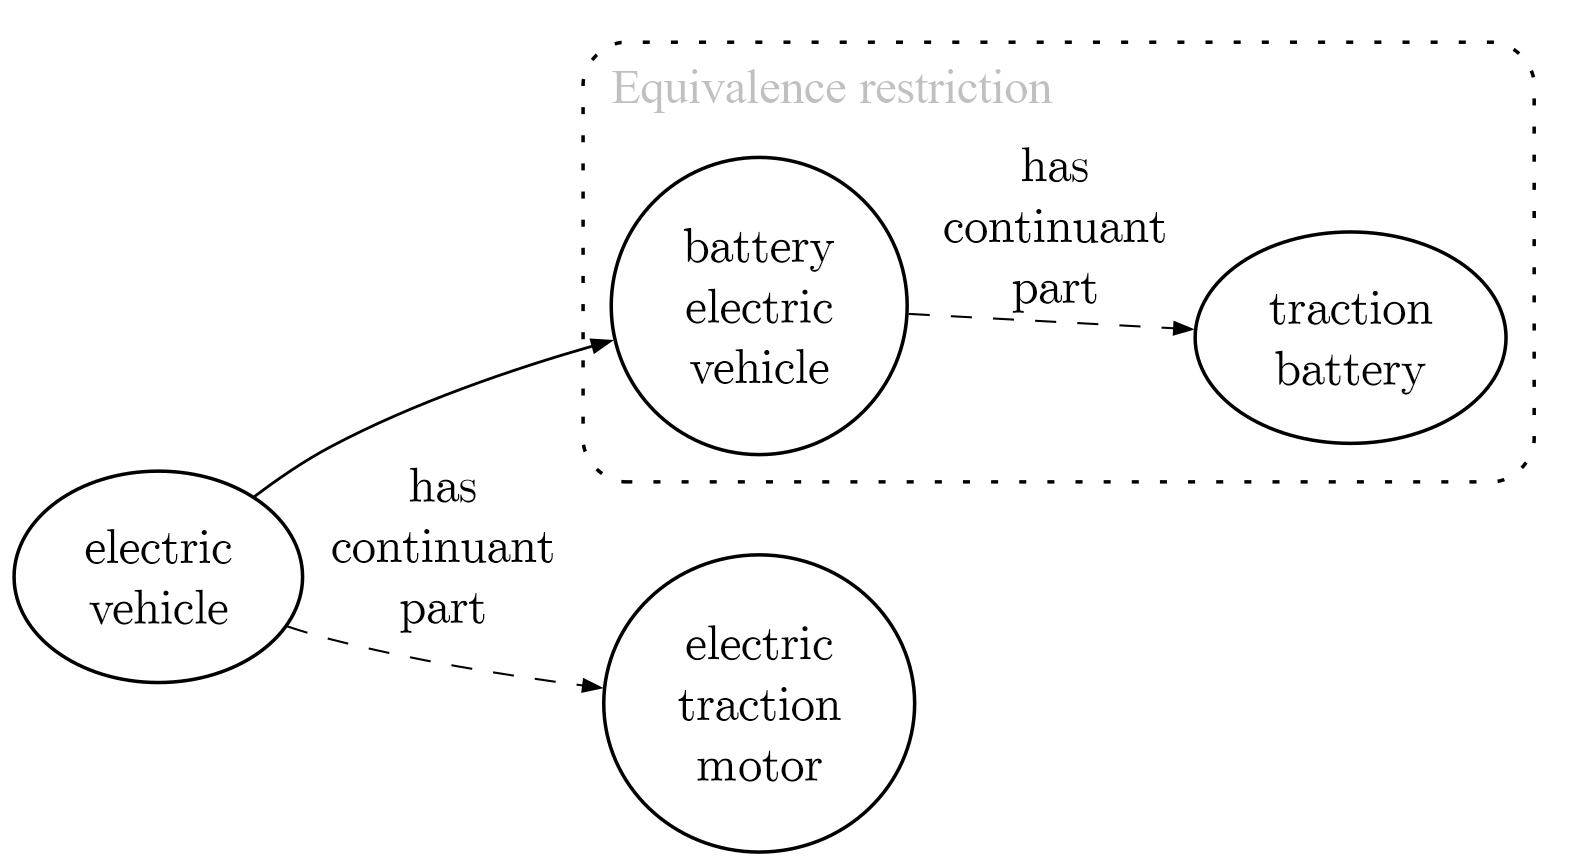
\includegraphics[width=1.0\textwidth]{images/OEOEV}
\end{figure}

\begin{figure}[h]
    \caption{Open energy ontology electric vehicle taxonomy.}
    \centering
    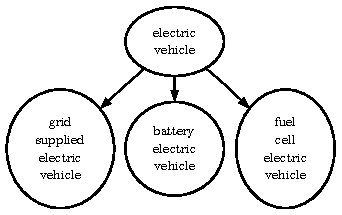
\includegraphics[width=0.9\textwidth]{images/OEOVehicles}
\end{figure}

\subsection{The Common Core Ontologies}

CCO section keywords: Infrastructure, Facilities Vehicle taxonomy

\begin{figure}[h]
    \caption{OEO Vehicle Taxonomy.}
    \centering
    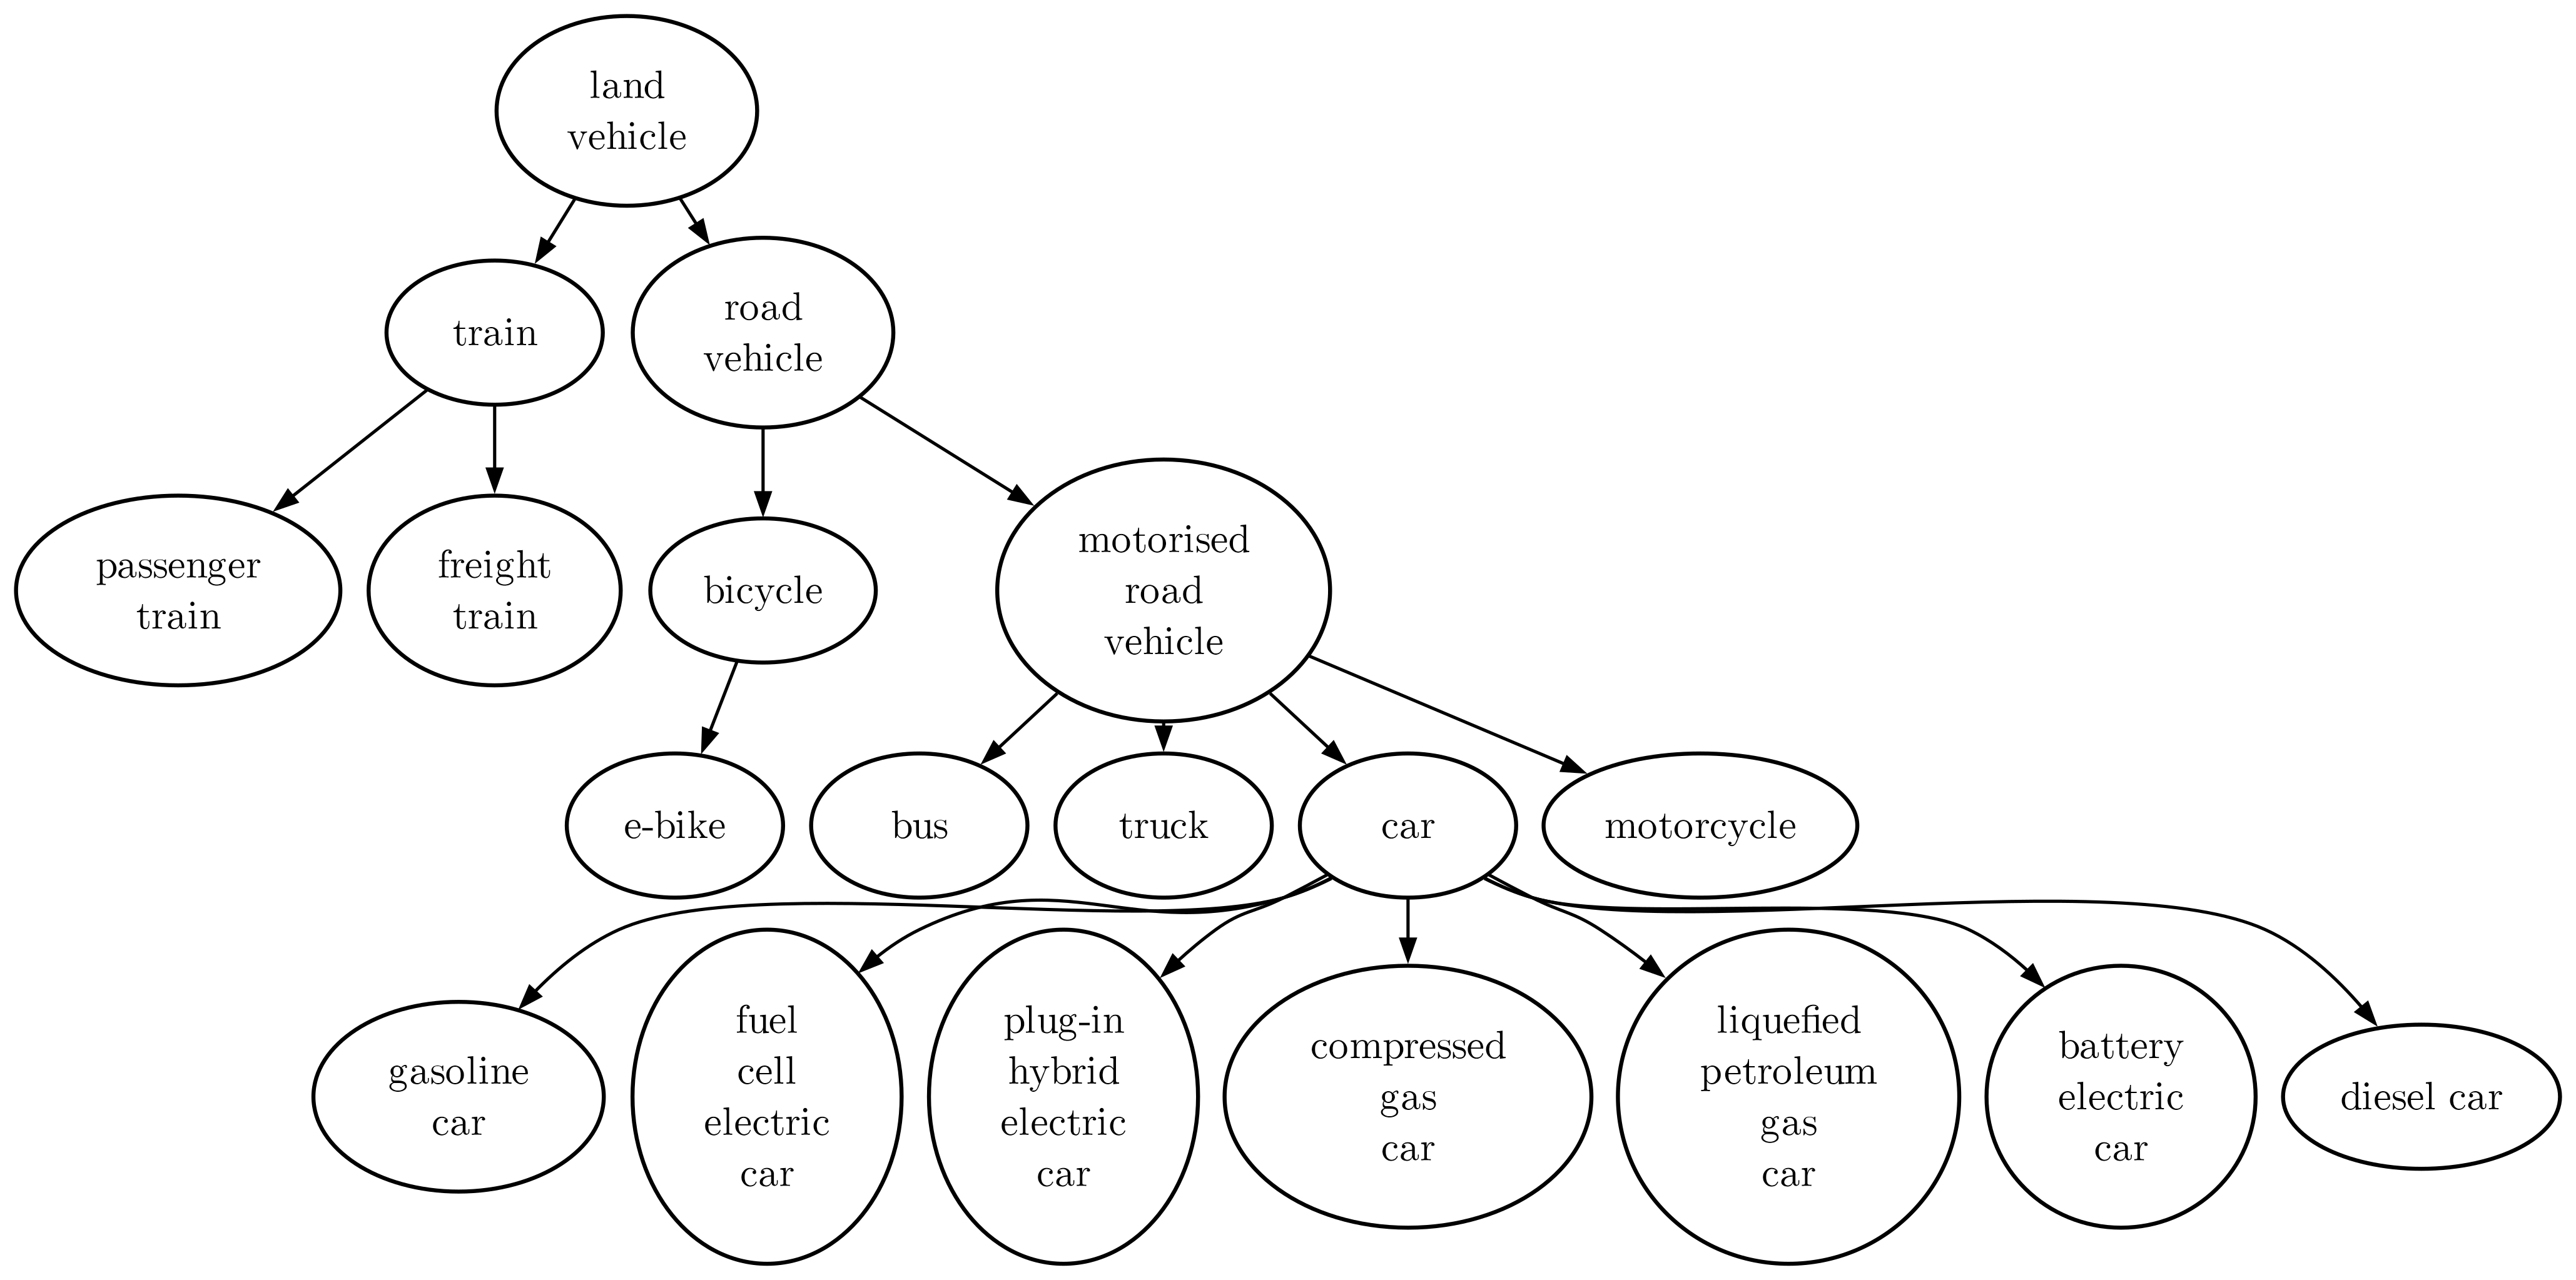
\includegraphics[width=0.9\textwidth]{images/OEOLVehicles}
\end{figure}

\begin{figure}[h]
    \caption{Common Core Ontologies Vehicle Taxonomy.}
    \centering
    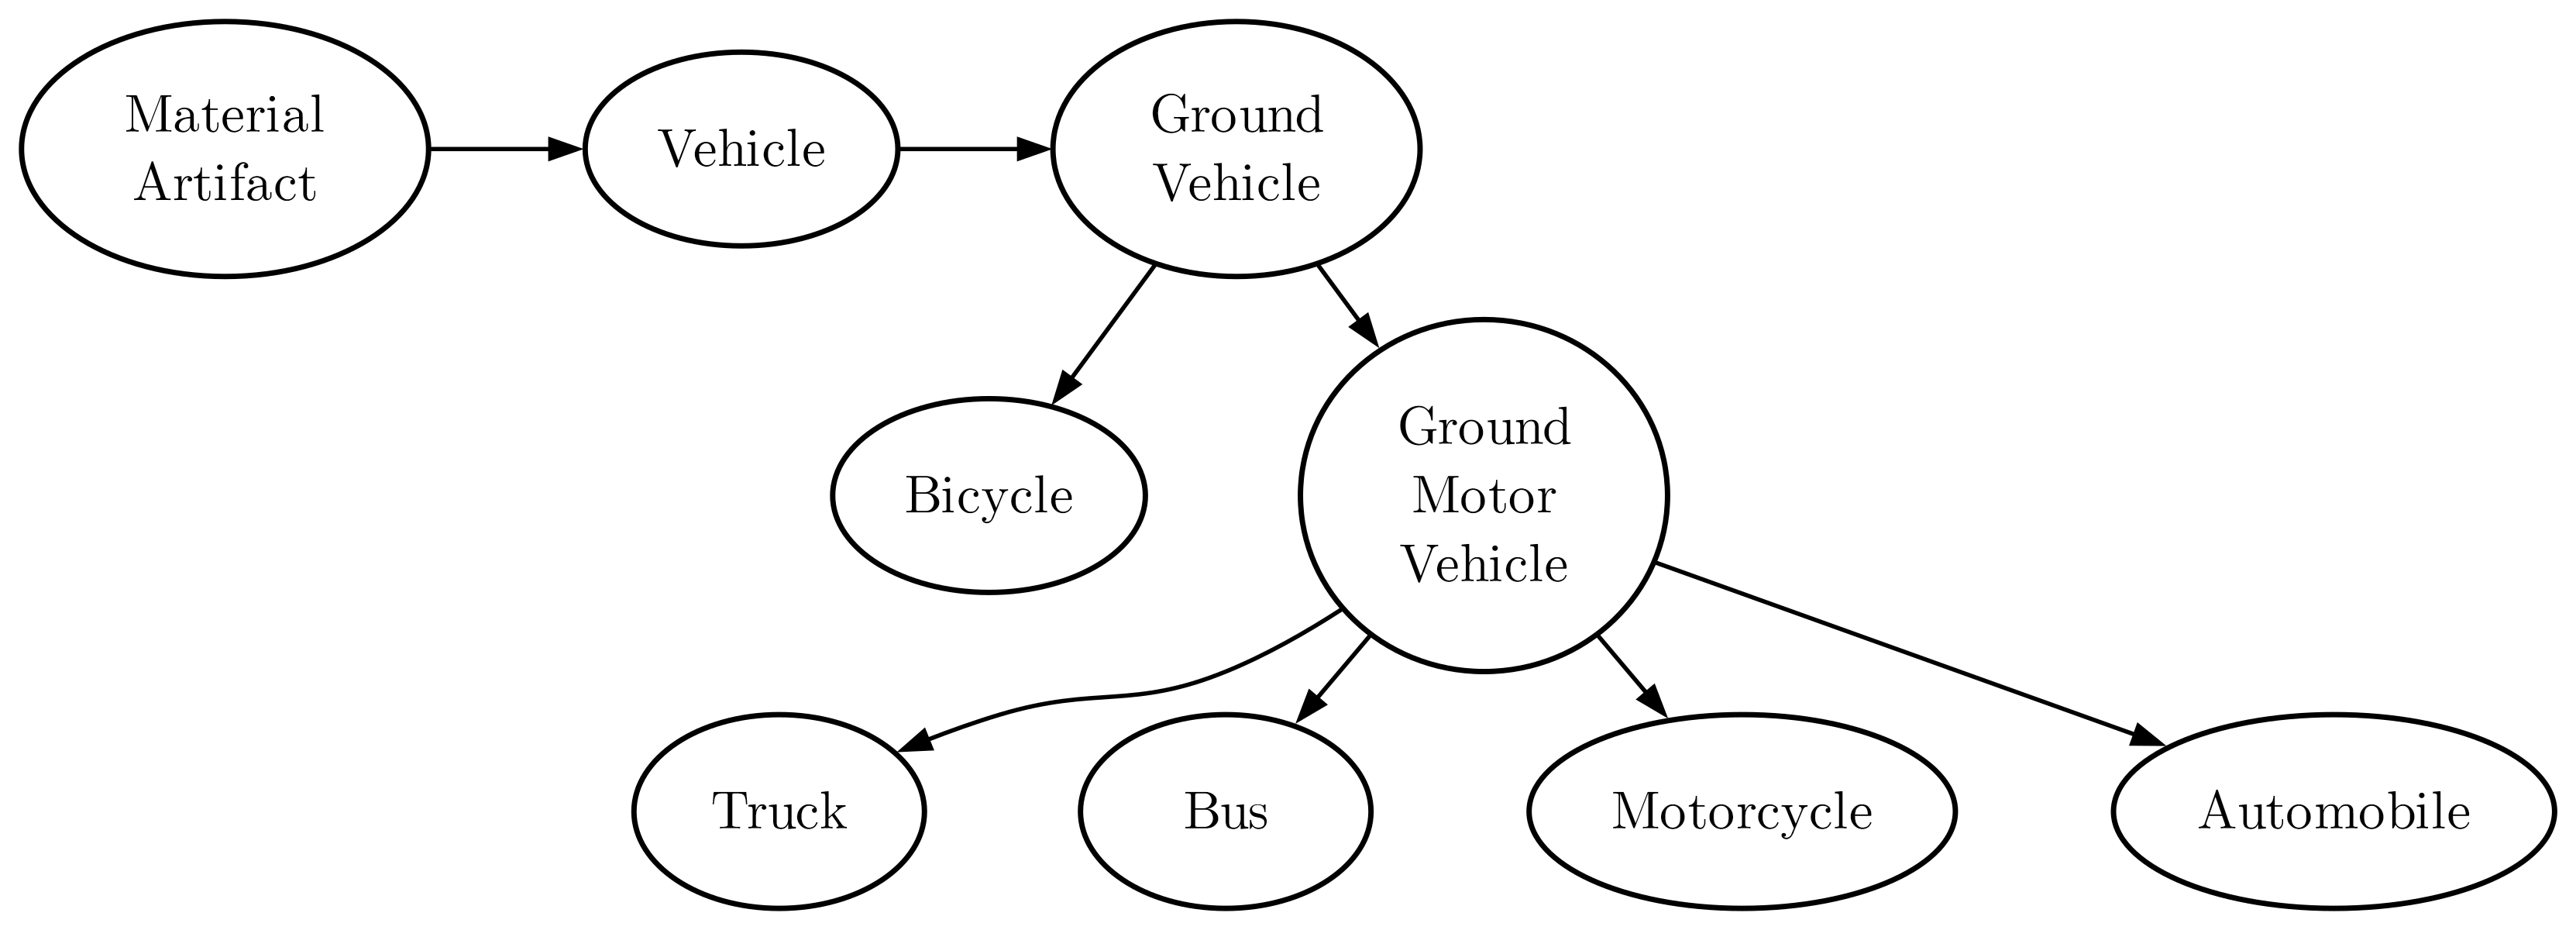
\includegraphics[width=0.9\textwidth]{images/CCOVehicles}
\end{figure}


\begin{figure}[h]
    \caption{Common Core Ontologies infrastructure constraints.}
    \centering
    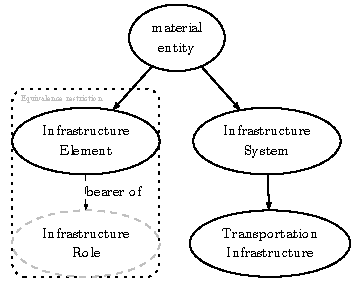
\includegraphics[width=1.0\textwidth]{images/infrastructureSystem}
\end{figure}



\subsection{iCity Parking ontology}

Parking section, keywords: Application specific, different Spatio-temopral assumptions

\begin{figure}[h]
    \caption{iCity parking ontology commitments associated to charging infrastructure.}
    \centering
    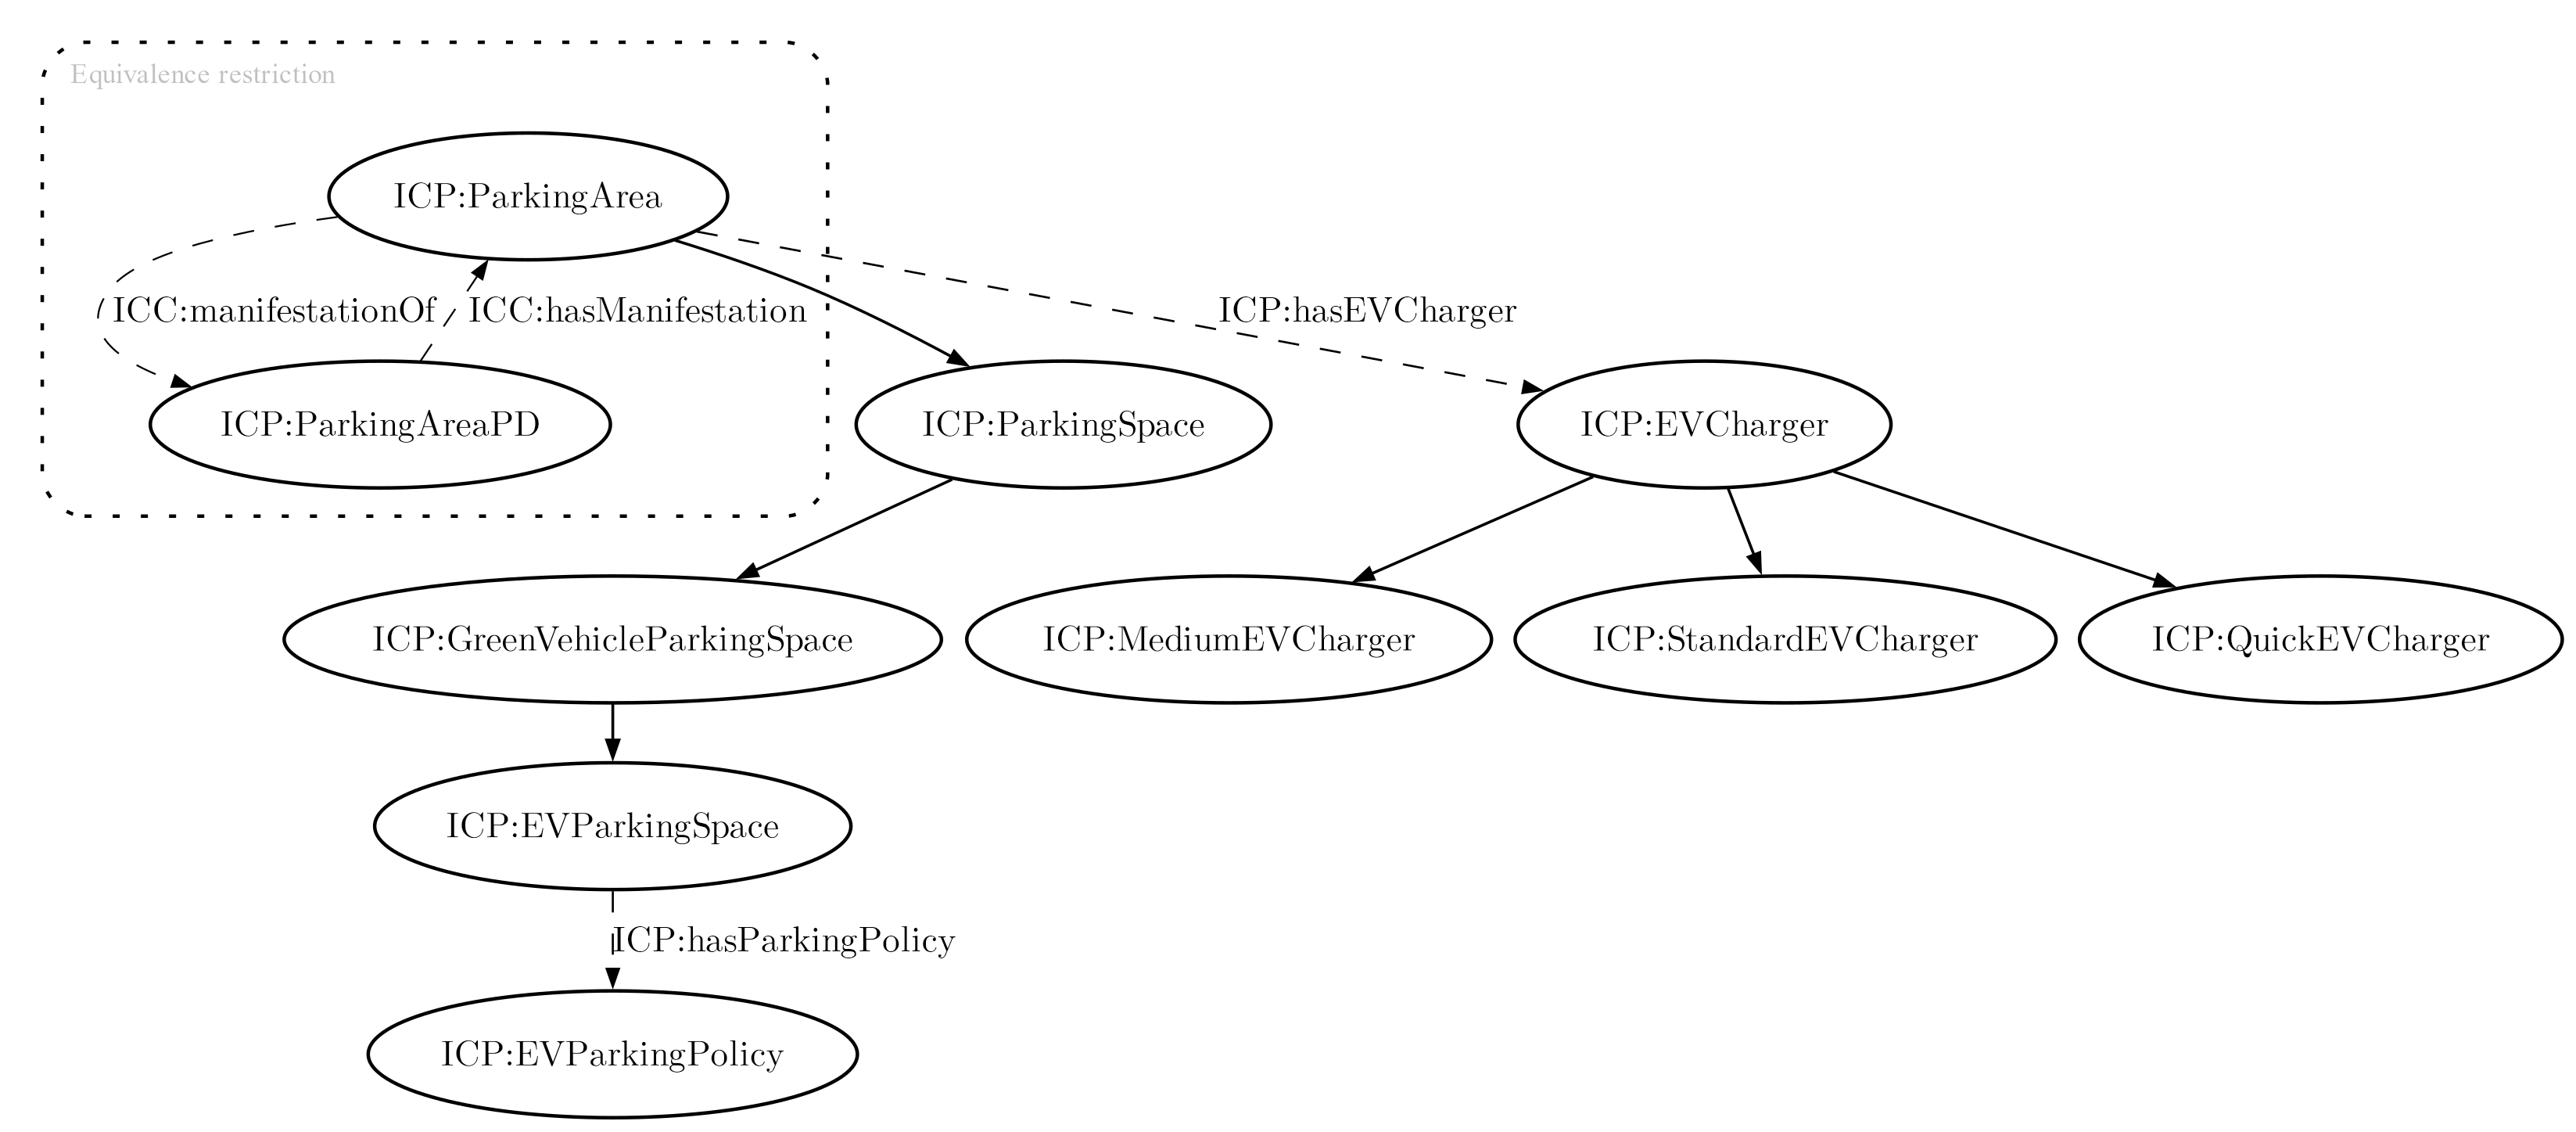
\includegraphics[width=1.0\textwidth]{images/PARKING}
\end{figure}
